\documentclass[%
 reprint,
%superscriptaddress,
%groupedaddress,
%unsortedaddress,
%runinaddress,
%frontmatterverbose, 
%preprint,
%preprintnumbers,
%nofootinbib,
%nobibnotes,
%bibnotes,
 amsmath,amssymb,
 aps,
%pra,
%prb,
%rmp,
%prstab,
%prstper,
floatfix,
]{revtex4-2}

\usepackage{graphicx}% Include figure files
\usepackage{dcolumn}% Align table columns on decimal point
\usepackage{bm}% bold math
\usepackage{kotex}
\usepackage{tabularx,ragged2e}
\usepackage{tabularray}
\usepackage{float} % H place indicator for figure and table
\usepackage{dblfloatfix}
\usepackage{subcaption}
\usepackage{hyperref}
\usepackage{array, makecell}

\setcellgapes{4pt}
\hypersetup{
  linkbordercolor=1 1 1,
  urlbordercolor=1 1 1,
  pdfauthor=author
}
\hbadness=99999
\vbadness=99999 

\newcolumntype{C}{>{\Centering\arraybackslash}X}

\graphicspath{ {./images/} }

\begin{document}

\title{\textbf{The Road to Muon Detection: Signal Amplifier and Peak Counter}}
\author{
    Woojin Han\textsuperscript{1}, Taeyoon Kim\textsuperscript{1}, Leo Park\textsuperscript{2}, Seokwon Song\textsuperscript{1}  \\
  \textsuperscript{1}Department of Physics \& Astronomy, Seoul National University, Seoul 08858, Korea \\
  \textsuperscript{2}Department of Mechanical Engineering , Seoul National University, Seoul 08858, Korea \\
  \date{\today}
}

\date{\today}

\begin{abstract}
    In this report, we designed and tested a signal amplification and peak detection circuit using operational amplifiers (op-amp) to detect signals such as those generated by muons.
    The experiment aimed to verify the circuit's ability to accurately identify the peaks of input signals while effectively suppressing noise.
    The peak detection circuit uses an op-amp, diode, capacitor, and resistors to capture and hold the maximum value of an input signal.
    The experimental setup used an Analog Discovery 2 to provide AC voltage, and measurements were taken over a range of frequencies from 2Hz to 200Hz and amplitudes from 0V to 2.5V.
    The results demonstrated that the peak detection circuit maintained a linear relationship between input and output voltages at lower frequencies, effectively capturing signal peaks.
    At higher frequencies, the circuit flattened the output signal, which leads us to reconstrain the redundant peak signals by modifying time windows.
    Moreover, the high frequency noise signals are also be negliable via this circuit.
    The combined circuit, which included both amplification and peak detection stages, also performed well, amplifying the input signal and maintaining accuracy across different frequency ranges.
    Additionally, the circuit successfully identified peaks in noise, with the diode automatically filtering out unnecessary signals, ensuring reliable and clean signal detection.
    These findings ensures the circuit's capability for precise signal measurement in applications like muon detection, which is our final project aim, identification and noise handling are well purposed.
\end{abstract}
\keywords{Suggested keywords}%Use showkeys class option if keyword
                              %display desired
\maketitle
\section{Introduction}
\subsection{OP amps}
\begin{figure}[H]
    \centering
    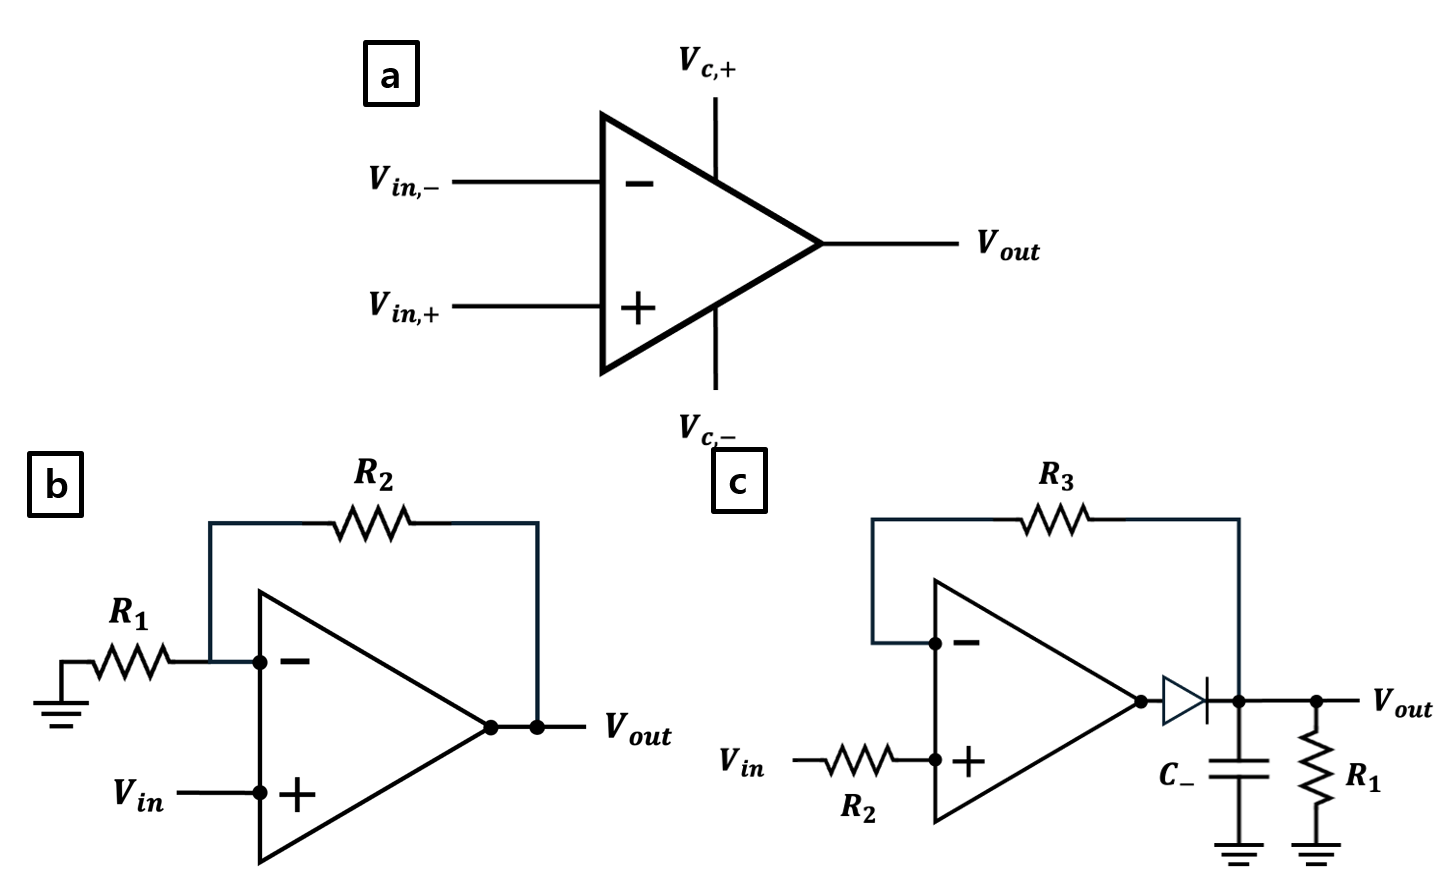
\includegraphics[width=0.4\textwidth]{total_circuits.png}
    \caption{
        (a) Schematic Operational Amplifier
        (b) Non-inverting Amplifier
        (c) Peak Detection Circuit
    }
    \label{fig: total_circuit_fig}
\end{figure}
Operational amplifiers, commonly referred to as op-amps, are fundamental building blocks in analog electronics, widely utilized in various applications ranging from signal amplification to complex mathematical operations.
An op-amp typically consists of a differential input stage, a high-gain amplification stage, and a low output impedance, which together enable it to amplify input voltage differences with high precision and stability.
One important design principle in op-amp circuits is the “10x rule,” which suggests that the input impedance of each stage should be at least ten times the output impedance of the preceding stage.
This guideline minimizes signal loss, ensures proper signal transfer, and reduces loading effects between stages, thereby maintaining the fidelity of the signal across multiple circuit stages.
Adherence to the 10x rule is especially critical in cascading amplifier stages, where even slight mismatches in impedance can lead to degradation in performance, signal distortion, and reduced gain accuracy.
By leveraging the high input impedance and low output impedance characteristics of op-amps, engineers can design circuits that meet these criteria, optimizing for both signal integrity and power efficiency.

For this experiment, two circuits employing op-amps are used for different purposes: amplification and peak detection.
In general, if the closed-loop system consists of op-amps, the two input voltages are matched due to the high input impedance and feedback characteristics.

The circuit shown in Fig. \ref{fig: total_circuit_fig} (b) is a non-inverting amplifier, which uses an operational amplifier (op-amp) to amplify the input signal \( V_{in} \) without changing its phase.
This configuration is called "non-inverting" because the output voltage \( V_{out} \) is in phase with the input, meaning there is no 180° phase shift as there would be in an inverting amplifier.
The input signal is applied to the non-inverting terminal (\(+\)) of the op-amp, while a feedback network composed of resistors \( R_1 \) and \( R_2 \) sets the amplifier's gain.
To derive the gain, we note that due to the high input impedance of the op-amp, the voltage at the inverting terminal (\(-\)) equals the input voltage \( V_{in} \) because of the virtual short concept.
The inverting terminal voltage \( V_{-} \) can also be described by the voltage divider formed by \( R_1 \) and \( R_2 \), giving \( V_{-} = V_{out} \cdot \frac{R_1}{R_1 + R_2} \).
Since \( V_{-} = V_{in} \), we have \( V_{in} = V_{out} \cdot \frac{R_1}{R_1 + R_2} \).
Rearranging this to express \( V_{out} \) in terms of \( V_{in} \) yields \( V_{out} = V_{in} \cdot \frac{R_1 + R_2}{R_1} \), so the gain \( A_v \) of the amplifier is \( A_v = \frac{V_{out}}{V_{in}} = 1 + \frac{R_2}{R_1} \).
This gain expression shows that the output is a scaled version of the input, with the scaling factor determined by \( R_1 \) and \( R_2 \), allowing for controlled amplification while preserving the input phase.


The circuit shown in Figure \ref{fig: total_circuit_fig} (c) is a peak detector designed to capture and hold the maximum voltage of an input signal \( V_{in} \), utilizing an operational amplifier, diode \( D \), capacitor \( C \), and resistors \( R_1 \), \( R_2 \), and \( R_3 \).
This configuration allows the circuit to record the highest input value at \( V_{out} \) without being affected by subsequent lower values.
The input voltage \( V_{in} \) is applied to the non-inverting terminal of the operational amplifier through resistor \( R_2 \), while feedback resistor \( R_3 \) sets the gain of the op-amp, ensuring that it drives the diode \( D \) with enough current to respond to small changes in \( V_{in} \).
When \( V_{in} \) reaches a new peak, the op-amp output forward-biases the diode \( D \), allowing current to charge the capacitor \( C \) to this peak value.
This charged voltage on \( C \) holds the peak value, as the diode prevents the capacitor from discharging through the op-amp when \( V_{in} \) drops below the peak.
The resistor \( R_1 \) provides a controlled discharge path, allowing the stored voltage on \( C \) to decay gradually over time if no higher peaks are encountered.
Consequently, the output voltage \( V_{out} \), taken across \( C \) and \( R_1 \), represents the peak of \( V_{in} \) until a new higher peak is detected or the stored voltage decays. (\cite{sedra_smith})

\subsection{Scintillator and SiPM}
\begin{figure}[H]
    \centering
    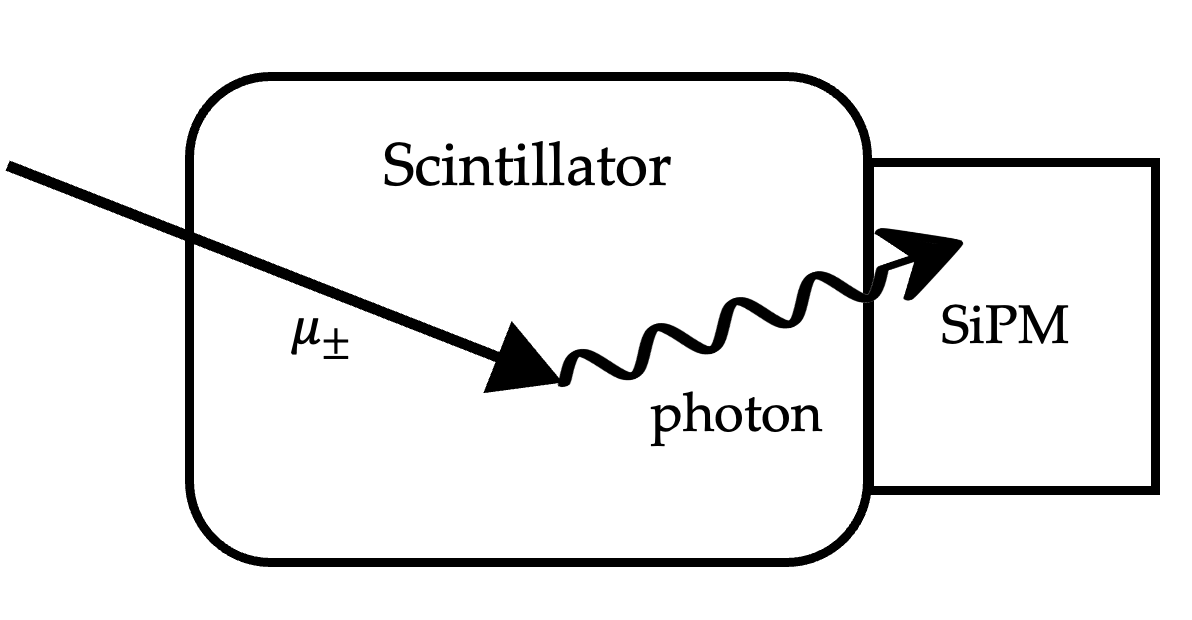
\includegraphics[width=0.4\textwidth]{scintillator.png}
    \caption{
        Schematic diagram of scintillator and SiPM detecting module
    }
    \label{fig: scintillator}
\end{figure}
Scintillator and SiPM are 2 main elements for detecting muons.
To understand its mechanism, it is crucial to know how muons behave in this setting.
First step is to know the origin of muons.
Cosmic rays, which are various kinds of radioactive high energy ray from the space, strike the atmosphere at every moment.
A very basic example would be the solar wind. To explain briefly, particles(such as pions) from cosmic rays react with atoms in the atmosphere, resulting high-energy muons.
Although muons naturally have a very short lifetime, the time dilation due to their fast speed allows them to reach the ground.
An exact reaction equations are at equation \ref*{eqn:rxn1} and \ref*{eqn:rxn2}. The particles in the equations are, respectively, pions, muons and muon neutrinos. 

\begin{equation}
  \label{eqn:rxn1}
  \pi^+ \rightarrow \mu^+ +\nu_\mu
\end{equation}
\begin{equation}
  \label{eqn:rxn2}
  \pi^- \rightarrow \mu^- +\overline{\nu_\mu}
\end{equation}

The main property of scintillator is that, when irradiated, it emits light.
When a muon (or any charged particle) strikes the scintillator, it interacts with molecules through electronic interactions.
The kinetic energy of muons would be transferred to the energy of electrons in these molecules.
The excited electrons will soon decay back to their original energy state, making a simultaneous light emission.
According to the law of energy conservation, the number of emitted photons is proportional to the given kinetic energy of the particle.
Simply put, scintillator is a substance that converts charged particles into light signals. (\cite{MuonDetection2023})

However, some noise signals may exist.
For example, alpha rays, beta rays and Compton scattered electrons from gamma rays can produce noise.
Although such noise is statistical in nature, the typical energy scales of these rays are known.
Muon's energy scale is about $50 \mathrm{MeV}$, whereas other particles typcally have energies around $1 \mathrm{MeV}$. (\cite{griffiths2008introduction})
Hence, one can deduce that the ratio between the signal and noise is $1/50$. 

The next step is to detect the emitted light from the scintillator. 
However, the luminosity of this light is very low and concentrated over a very short period of time. 
SiPM is the sensor designed to capture such light signals.
Quantitatively, a muon signal lasts on the scale of several microseconds, while SiPM can capture signals on the nanosecond scale.
In this experiment, we will use SiPM to collect the muon signal.
At this level of detection, noise is also present.
The SiPM has it own inherent noise, known as the dark rate.
In the SiPM, the charge carriers generate signals by transition between conduction/valence band or two distinct bands.
Usually such transition is given by light (in other words, electronic field), but also thermal noise would make a defect on the output signal.
Such noise depends on the temperature of the system.


\section{Experiment}
\subsection{Apparatus and Codes}
The AC voltage in this experiment was provided by Analog Discovery 2. (\cite{K_AnalogDiscovery2})

\subsection{Peak Detection Circuit}
The peak detection circuit, as shown in Fig. \ref{fig: total_circuit_fig} (c), was constructed using an op-amp, a diode, a capacitor and two resistors with $R_3=988.0\pm0.05k\Omega$, $R_5=99.57\pm0.05k\Omega$ and $C=4.599\pm0.0005\mu F$.
An AC voltage was provided as an input sinusodial signal which was expected to be detected by the peak detection circuit.  
The nodes between the drive AC voltage and the output detection signal were connected to Channel 1 and Channel 2 of Analog Discovery 2 Oscilloscope, respectively. 
A total of 20 measurements were taken over the frequency range of $2\mathrm{Hz}$ to $200\mathrm{Hz}$ on a logarithmic scale.  
For each frequency, measurements were taken at intervals of $0.05\mathrm{V}$ over the input signal's amplitude range of $0\mathrm{V}$ to $2.5\mathrm{V}$. 
All data were measured for a duration of 10 periods. \\
The waveforms of the input and output signals were compared to verify whether the peak of the sinusodial signal was properly detected for each frequency. 
Also, minimum and maximum voltage of the input and output signal were measured by period. 
The linear relationship between the input and output signals' voltage was analyzed for each minimum and maximum voltage, respectively. 
Also using that, their gain, a ratio between input and output signal voltage for minimum and maximum value were also calculted. 
Then, the variation of gains of minimum and maximum voltage with respect to frequency were investigated.
\\

\subsection{Total Circuit}
The entire circuit consists of an amplification circuit, as shown in Figure 1, and a peak detection circuit, as shown in Figure 2.
The resistors with $R_1=465.9\pm0.05\Omega$, $R_2=46.98\pm0.005\Omega$ were used in an amplification circuit and a capacitor, resistors in a peak detection circuit was the same as above. 
The node were connected same as above also. 
Measurements and analysis of results were carried out in the same manner as the previous peak detection circuit experiment.

\section{Results}
 The subsections includes four experimental results.
 In \ref{Subsection: Results of Single Circuit}, the performance of the peak detection circuit is depicted.
 The experiment was held in the frequency, amplitude region of $2 \mathrm{Hz} ~ 200 \mathrm{Hz}$, and $0 ~ 2.5 \mathrm{V}$ is plotted.
 The time dependent plot of input and output signal is provided with minimum voltage gain via drive voltage is linearly regressed.
 Therefore, the measured error assumes the peak detection is well working for all frequency window we aimed for. 
 In \ref{Subsection: Results of Total Circuits}, the frequency and amplitude sweep results from $2 \mathrm{Hz} ~ 200 \mathrm{Hz}$, and $0 ~ 0.25 \mathrm{V}$ is provided.
 The lineary successful profile of each circuit, and the integrable nature is experimentally proven.
 Finally, in \ref{Subsection: Response to Noise Profile} the total circuit are tested in noisy peak input to prove its capability in real expected output of photon multiplier.
 The time constant of the circuit are easily modifiable, which takes part of the peak detecting time threshold of signal with noise. 

\subsection{Peak Detection Circuit}
\label{Subsection: Results of Single Circuit}
The peak detection circuit widely spreads the input signals in time constant of the circuit.
In this experiment, the time constant of the AC handling component is $0.458 [s]$ which are induced by the measured resistance and capacitance value.
As we can see in Fig. \ref{fig: Peak Detection Results}(a) and (b), contains the input signal (black dots) and output signal (red dots) of the circuit in function of time.
While the input signal drives the circuit, the diode constrains the charging direction, the output signal is ruled by the number of peaks of the signal.
To numerize the result, the minimum and maximum voltage via time is used.
The maximum voltage of output signal gives the information of the size of the drive signal, and the difference between minimum and maximum voltage provides the number of relavent peaks in time window.
Fig. \ref{fig: Peak Detection Results} (c) shows the linear nature of the signal gain while the driving voltage changes.
The value of min/max voltage in driving amplitude, and its linear regression results shows that in same frequency, the input voltage is linearly dependent to the output signal.
Fig. \ref{fig: Peak Detection Results} (d) shows the linear regression coefficients by the frequency of the input signal.
As the frequency increases, the gain of minimum and maximum signals are converged to the same value, which implies that the peak detection circuit gives flat signal when the change of the signal is way more rapid than the time constant what we have set.

\begin{figure}[H]
    \centering
    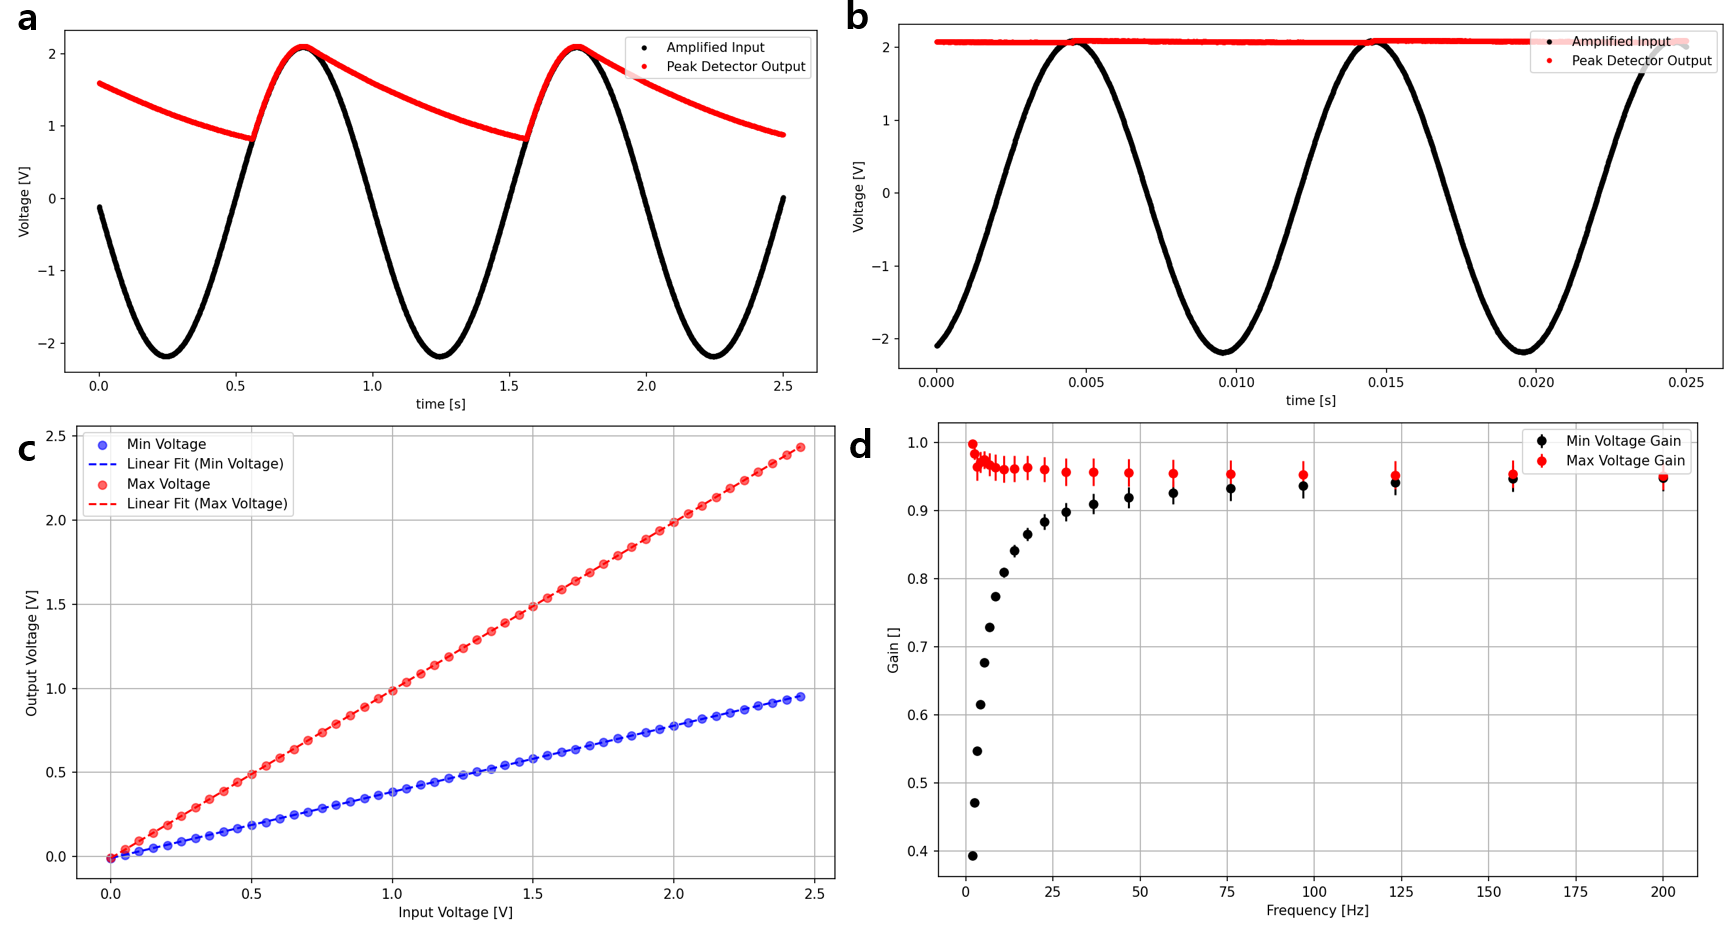
\includegraphics[width=0.4\textwidth]{./images/peak_detection_results.png}
    \caption{
        (a) time[s] - voltage [V] result for $2 \mathrm{V}$, $1 \mathrm{Hz}$ drive which are in black dots plotted, with output signal in red dots.
        (b) time[s] - voltage [V] result for $2 \mathrm{V}$, $100 \mathrm{Hz}$ drive respectively.
        (c) output voltage [V] - input voltage [V] of the minimum and maximum voltage of the output signal is plotted each in red and blue dots.
        The line in each color represents the linear regresssion result in voltage.
        (d) Gain - input frequency [Hz] of the total experiment results. the Gain of each minimum and maximum voltages are obtained by linear regression.
    }
    \label{fig: Peak Detection Results}
\end{figure}

\subsection{Total Circuit Results}
\label{Subsection: Results of Total Circuits}
The total circuit passes the amplified input signal through the amplification circuit, which then detects the peak through the peak detection circuit. 
Similar with the result of the peak detection circuit, Fig. \ref{fig: Total Circuit Results} (a) demonstrates the linearity of the signal gain with respect to the voltage of the input signal. 
The both max/min gain shows the linearity similar with the result of the peak detection circuit. 
On the other hand, an expected gain of the amplification circuit is $A_v=10.92$ which is calculated by the measured resistance values. 
Since the results were measured in the 0 to 0.25V input voltage range, it can be confirmed that the amplification circuit is also operating properly.
Fig.\ref{fig: Total Circuit Results} (b) shows the linear regression coefficients by the frequency of the input signal for the total circuit. 
The similar tendency to the peak detected circuit was also observed in the total circuit which contains the amplification circuit. 
Therefore, the total circuit, the circuit one would use in the final project about a muon detection, also gives a flat signal when the change of the signal is way more rapid than the time constant what we have set. 
In contrast, for the low frequency signal, a difference between max/min gain is much bigger. 
Since signals of muons consist of peaks and noises which are correspoding to low and high frequency signals, this total circuit is considered suitable for detecting the energy signal of muons in the final project.
\begin{figure}[H]
    \centering
    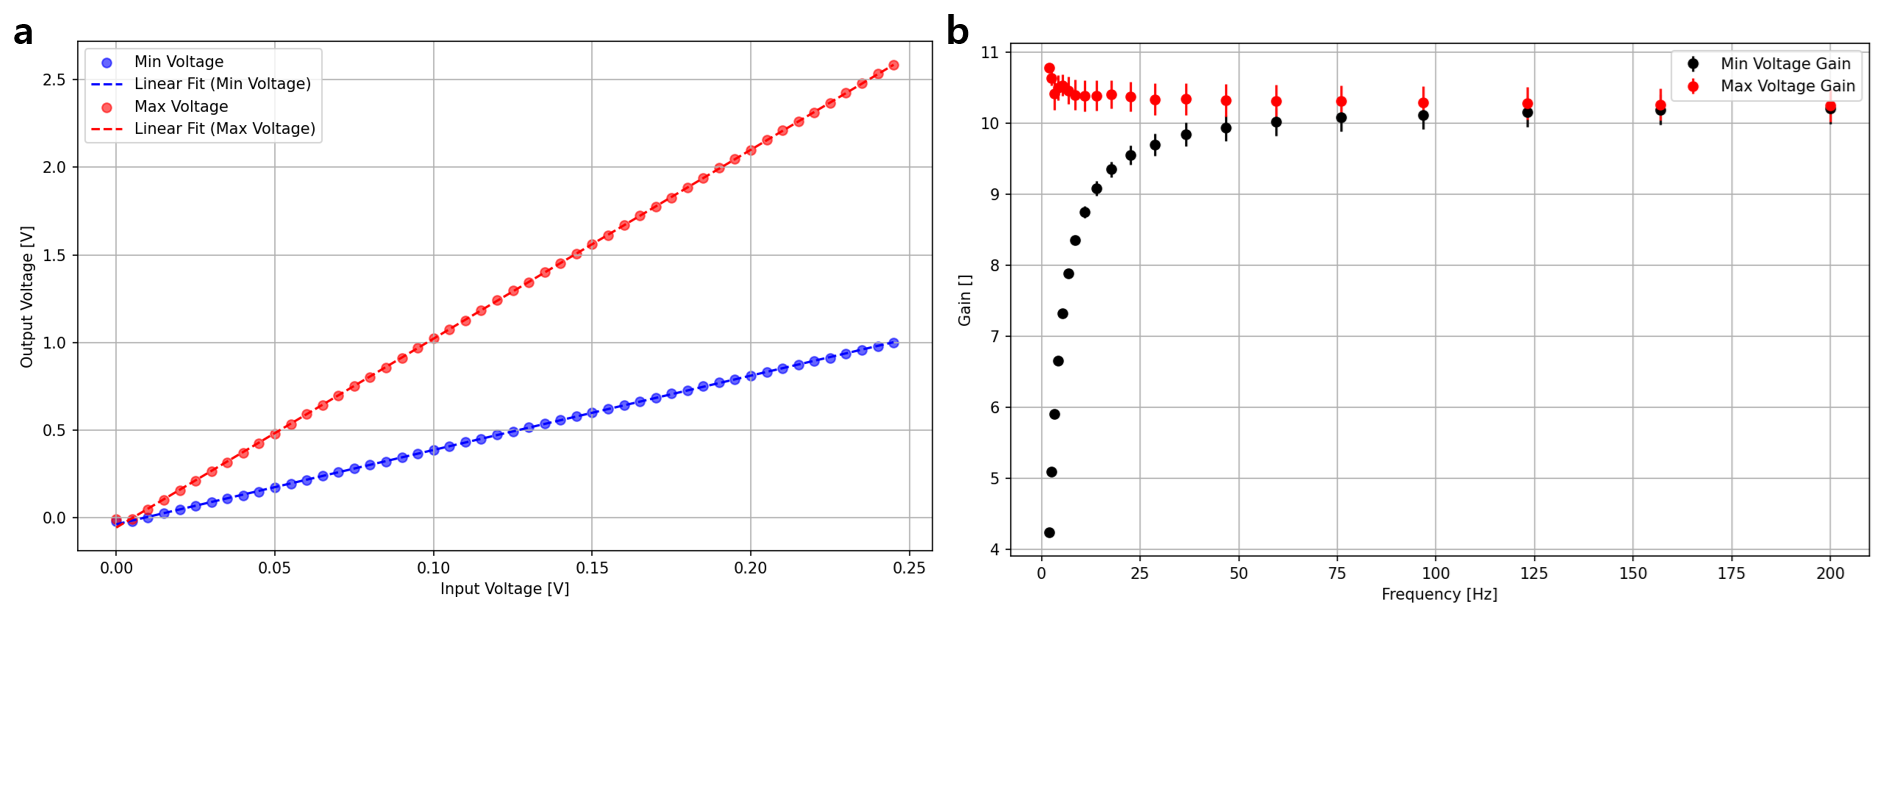
\includegraphics[width=0.4\textwidth]{./images/total_circuit_results.png}
  \caption{
      (a) output voltage [V] - input voltage [V] of the minimum and maximum voltage of the output signal is plotted each in red and blue dots.
      The line in each color represents the linear regresssion result in voltage.
      (b) Gain - input frequency [Hz] of the total experiment results. The Gain of each minimum and maximum voltages are obtained by linear regression.
  }
  \label{fig: Total Circuit Results}
\end{figure}


\subsection{Response to Noise Profile}
\label{Subsection: Response to Noise Profile}
 The muon creates the peak with degenerate noises.
 In degenerate thermal noise, the muon peak have $S/N$ ratio above 30, in few $\mu s$.
 Therefore, the circuit we have should detect the peak provided in very short time, surrounded by the noise background.
 To test the performance in response on the signal, we created certain signal by AD2.
 Fig. \ref{fig: Noise Response Results} shows the signal and its response of total circuit.
 As expected the peaks are easily countable when the signal takes time difference in order of time constant of the circuit.
 In this case, the constant of the circuit is about $500 ms$.
 By the muon decay, the single muon creates a dozens of peaks.
 Therefore, the appropriate set of the time window is mandetory.
 Fig. \ref{fig: Noise Response Results}(b) shows that redundant peaks inbetweens are vanishes automatically by the diode in the circuit, and creates clean countable signal.
 \begin{figure}[H]
    \centering
    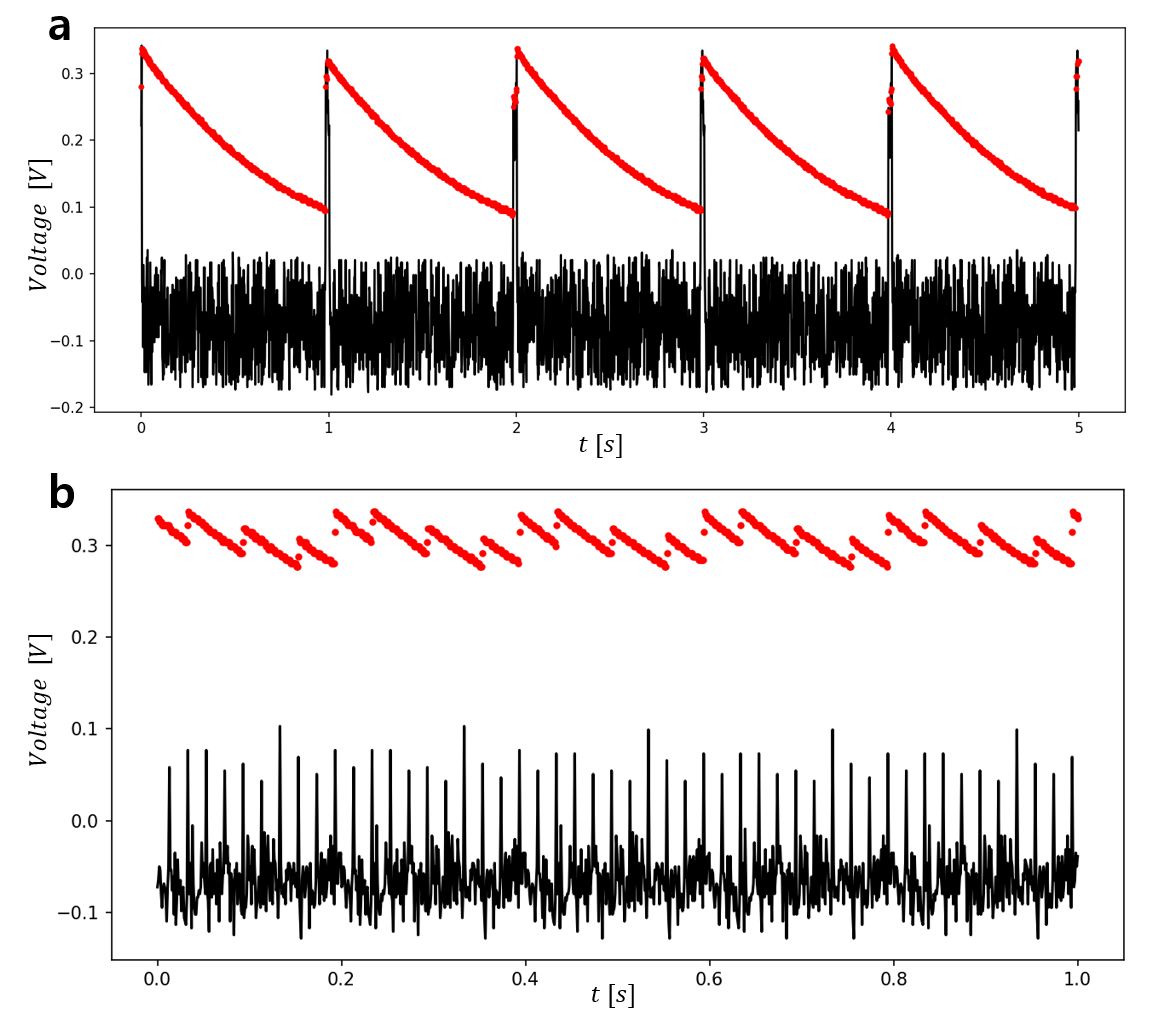
\includegraphics[width=0.4\textwidth]{./images/noise_response.png}
    \caption{
        The black line shows the peak with noise, and the red dots shows the output signal of total circuit.
        The experimental setting varies,
        (a) time[s] - voltage [V] result for signal $0.3 \pm 0.1 \mathrm{V}$, $1 \mathrm{Hz}$.
        (b) time[s] - voltage [V] result for signal $0.2 \pm 0.1 \mathrm{V}$, $50 \mathrm{Hz}$
    }
    \label{fig: Noise Response Results}
  \end{figure}
\section{Discussion}
The experiment showed that the peak detection circuit worked well, accurately identifying signal peaks and maintaining a linear relationship between input and output voltages.
It performed well in  lower frequencies, so that the peak gives the higher signals after the circuit.
The noise signal, in high frequencies, flattened out as the circuit is linearly well performing.
When combined with an amplifier in the total circuit, the setup maintained good performance, amplifying signals without propagating errors.
The total circuit worked well across different frequencies and proved good outputs both amplification and peak detection, such as measuring photonic signals from muons.
Finally, testing with noisy signals showed the total circuit could still identify important peaks, making it effective in muon detections.
By using a diode, the circuit automatically removed unnecessary peaks, ensuring accurate and clean signal detection.
The time window of the screening signals are anlogly controlled by the time constant of AC component.
Overall, these circuits are reliable and suitable for applications requiring precise signal measurement and noise handling.
\section{References}
\bibliographystyle{plain} 
\bibliography{pkdtref}


\end{document}